\documentclass[11pt,a4paper]{ctexart}
% Shared preamble for the assignment reports. Use with:
%   \documentclass[11pt,a4paper]{ctexart}  (XeLaTeX)
%   % Shared preamble for the assignment reports. Use with:
%   \documentclass[11pt,a4paper]{ctexart}  (XeLaTeX)
%   % Shared preamble for the assignment reports. Use with:
%   \documentclass[11pt,a4paper]{ctexart}  (XeLaTeX)
%   \input{../common/preamble.tex}
\usepackage[margin=2.3cm]{geometry}
\setmainfont{texgyretermes}[Extension=.otf,UprightFont=*-regular,BoldFont=*-bold,ItalicFont=*-italic,BoldItalicFont=*-bolditalic]
\setsansfont{texgyreheros}[Extension=.otf,UprightFont=*-regular,BoldFont=*-bold,ItalicFont=*-italic,BoldItalicFont=*-bolditalic]
\setmonofont{texgyrecursor}[Extension=.otf,UprightFont=*-regular,BoldFont=*-bold,ItalicFont=*-italic,BoldItalicFont=*-bolditalic]
\usepackage{amsmath,amssymb,mathtools,bm}
\usepackage{graphicx}
\usepackage{booktabs,multirow,makecell,array,tabularx}
\usepackage[table]{xcolor}
\usepackage[most]{tcolorbox}
\usepackage{enumitem}
\usepackage{listings}
\usepackage{subcaption}
\usepackage{siunitx}
\usepackage[hidelinks]{hyperref}
\usepackage[nameinlink,noabbrev]{cleveref}
\usepackage{float}

\setlength{\emergencystretch}{3em}
\linespread{1.15}
\setlist{leftmargin=*,itemsep=2pt,topsep=3pt}
\graphicspath{{figures/}}

\crefname{figure}{图}{图}
\crefname{table}{表}{表}
\crefname{section}{第}{第}
\creflabelformat{section}{#2#1#3 节}
\crefname{equation}{式}{式}
\crefformat{equation}{式~(#2#1#3)}

\lstset{basicstyle=\ttfamily\footnotesize,columns=fullflexible,breaklines=true,frame=single,
  framerule=0.3pt,rulecolor=\color{black!40},backgroundcolor=\color{black!3},
  keywordstyle=\color{blue!60!black}\bfseries,commentstyle=\color{green!40!black},
  numbers=left,numberstyle=\tiny\color{black!50},xleftmargin=1.5em}

% Interview boxes: question, model answer, common wrong answer.
\newtcolorbox{iqbox}[1]{enhanced,breakable,colback=blue!3,colframe=blue!45!black,boxrule=0.5pt,arc=1.5pt,
  left=4pt,right=4pt,top=3pt,bottom=3pt,fonttitle=\bfseries\small,title={面试追问：#1}}
\newtcolorbox{findingbox}[1][]{enhanced,breakable,colback=green!3,colframe=green!40!black,boxrule=0.5pt,arc=1.5pt,
  left=4pt,right=4pt,top=3pt,bottom=3pt,fonttitle=\bfseries\small,title={结论#1}}
\newtcolorbox{caveatbox}{enhanced,breakable,colback=orange!4,colframe=orange!60!black,boxrule=0.5pt,arc=1.5pt,
  left=4pt,right=4pt,top=3pt,bottom=3pt,fonttitle=\bfseries\small,title={不能推出的结论}}

\newcommand{\authorline}{ShaneLiu04\thanks{GitHub: \url{https://github.com/ShaneLiu04}。代码与原始指标见 edge-deploy 仓库各 lab 的 \texttt{artifacts/raw/}。本文基于公开课程材料独立完成，与课程团队无隶属关系。}}

\usepackage[margin=2.3cm]{geometry}
\setmainfont{texgyretermes}[Extension=.otf,UprightFont=*-regular,BoldFont=*-bold,ItalicFont=*-italic,BoldItalicFont=*-bolditalic]
\setsansfont{texgyreheros}[Extension=.otf,UprightFont=*-regular,BoldFont=*-bold,ItalicFont=*-italic,BoldItalicFont=*-bolditalic]
\setmonofont{texgyrecursor}[Extension=.otf,UprightFont=*-regular,BoldFont=*-bold,ItalicFont=*-italic,BoldItalicFont=*-bolditalic]
\usepackage{amsmath,amssymb,mathtools,bm}
\usepackage{graphicx}
\usepackage{booktabs,multirow,makecell,array,tabularx}
\usepackage[table]{xcolor}
\usepackage[most]{tcolorbox}
\usepackage{enumitem}
\usepackage{listings}
\usepackage{subcaption}
\usepackage{siunitx}
\usepackage[hidelinks]{hyperref}
\usepackage[nameinlink,noabbrev]{cleveref}
\usepackage{float}

\setlength{\emergencystretch}{3em}
\linespread{1.15}
\setlist{leftmargin=*,itemsep=2pt,topsep=3pt}
\graphicspath{{figures/}}

\crefname{figure}{图}{图}
\crefname{table}{表}{表}
\crefname{section}{第}{第}
\creflabelformat{section}{#2#1#3 节}
\crefname{equation}{式}{式}
\crefformat{equation}{式~(#2#1#3)}

\lstset{basicstyle=\ttfamily\footnotesize,columns=fullflexible,breaklines=true,frame=single,
  framerule=0.3pt,rulecolor=\color{black!40},backgroundcolor=\color{black!3},
  keywordstyle=\color{blue!60!black}\bfseries,commentstyle=\color{green!40!black},
  numbers=left,numberstyle=\tiny\color{black!50},xleftmargin=1.5em}

% Interview boxes: question, model answer, common wrong answer.
\newtcolorbox{iqbox}[1]{enhanced,breakable,colback=blue!3,colframe=blue!45!black,boxrule=0.5pt,arc=1.5pt,
  left=4pt,right=4pt,top=3pt,bottom=3pt,fonttitle=\bfseries\small,title={面试追问：#1}}
\newtcolorbox{findingbox}[1][]{enhanced,breakable,colback=green!3,colframe=green!40!black,boxrule=0.5pt,arc=1.5pt,
  left=4pt,right=4pt,top=3pt,bottom=3pt,fonttitle=\bfseries\small,title={结论#1}}
\newtcolorbox{caveatbox}{enhanced,breakable,colback=orange!4,colframe=orange!60!black,boxrule=0.5pt,arc=1.5pt,
  left=4pt,right=4pt,top=3pt,bottom=3pt,fonttitle=\bfseries\small,title={不能推出的结论}}

\newcommand{\authorline}{ShaneLiu04\thanks{GitHub: \url{https://github.com/ShaneLiu04}。代码与原始指标见 edge-deploy 仓库各 lab 的 \texttt{artifacts/raw/}。本文基于公开课程材料独立完成，与课程团队无隶属关系。}}

\usepackage[margin=2.3cm]{geometry}
\setmainfont{texgyretermes}[Extension=.otf,UprightFont=*-regular,BoldFont=*-bold,ItalicFont=*-italic,BoldItalicFont=*-bolditalic]
\setsansfont{texgyreheros}[Extension=.otf,UprightFont=*-regular,BoldFont=*-bold,ItalicFont=*-italic,BoldItalicFont=*-bolditalic]
\setmonofont{texgyrecursor}[Extension=.otf,UprightFont=*-regular,BoldFont=*-bold,ItalicFont=*-italic,BoldItalicFont=*-bolditalic]
\usepackage{amsmath,amssymb,mathtools,bm}
\usepackage{graphicx}
\usepackage{booktabs,multirow,makecell,array,tabularx}
\usepackage[table]{xcolor}
\usepackage[most]{tcolorbox}
\usepackage{enumitem}
\usepackage{listings}
\usepackage{subcaption}
\usepackage{siunitx}
\usepackage[hidelinks]{hyperref}
\usepackage[nameinlink,noabbrev]{cleveref}
\usepackage{float}

\setlength{\emergencystretch}{3em}
\linespread{1.15}
\setlist{leftmargin=*,itemsep=2pt,topsep=3pt}
\graphicspath{{figures/}}

\crefname{figure}{图}{图}
\crefname{table}{表}{表}
\crefname{section}{第}{第}
\creflabelformat{section}{#2#1#3 节}
\crefname{equation}{式}{式}
\crefformat{equation}{式~(#2#1#3)}

\lstset{basicstyle=\ttfamily\footnotesize,columns=fullflexible,breaklines=true,frame=single,
  framerule=0.3pt,rulecolor=\color{black!40},backgroundcolor=\color{black!3},
  keywordstyle=\color{blue!60!black}\bfseries,commentstyle=\color{green!40!black},
  numbers=left,numberstyle=\tiny\color{black!50},xleftmargin=1.5em}

% Interview boxes: question, model answer, common wrong answer.
\newtcolorbox{iqbox}[1]{enhanced,breakable,colback=blue!3,colframe=blue!45!black,boxrule=0.5pt,arc=1.5pt,
  left=4pt,right=4pt,top=3pt,bottom=3pt,fonttitle=\bfseries\small,title={面试追问：#1}}
\newtcolorbox{findingbox}[1][]{enhanced,breakable,colback=green!3,colframe=green!40!black,boxrule=0.5pt,arc=1.5pt,
  left=4pt,right=4pt,top=3pt,bottom=3pt,fonttitle=\bfseries\small,title={结论#1}}
\newtcolorbox{caveatbox}{enhanced,breakable,colback=orange!4,colframe=orange!60!black,boxrule=0.5pt,arc=1.5pt,
  left=4pt,right=4pt,top=3pt,bottom=3pt,fonttitle=\bfseries\small,title={不能推出的结论}}

\newcommand{\authorline}{ShaneLiu04\thanks{GitHub: \url{https://github.com/ShaneLiu04}。代码与原始指标见 edge-deploy 仓库各 lab 的 \texttt{artifacts/raw/}。本文基于公开课程材料独立完成，与课程团队无隶属关系。}}

\graphicspath{{../../solutions/mlc/tensor-program-tuning/artifacts/figures/}}

\newcommand{\sk}[1]{\texttt{#1}}

\title{MLC 张量程序调优实验报告：\\在 4 核 CPU 上自己做一遍 AutoTVM——调度空间、寄存器分块、代价模型、测量噪声与向量宽度}
\author{\authorline}
\date{2026 年 11 月}

\begin{document}
\maketitle

\begin{abstract}
MLC 课程（陈天奇）讲张量程序抽象与自动优化，TVM 的 AutoTVM / Ansor / MetaSchedule 把它做成了产品。本报告不依赖 TVM，自己实现整个闭环：
七个旋钮的调度空间 → 生成 C++ → 4 路并行 g++ 编译 → 严格顺序实测并对参考结果校验 → 四种搜索策略（grid / random / 代价模型引导 / 进化）各 3 个种子、每次 64 次实测
→ 岭回归代价模型的留出 Spearman → 前 8 名复测与 256 / 512 位向量对照。问题是 fp32 GEMM：$256^3$ 方阵（空间 30,240 个点），
以及 MobileNetV2 的 pw\_expand\_14（$196\times576\times96$，空间 3,888 个点）。主平台是 Ice Lake 4 核虚拟机（AVX-512，MinGW g++ 13.2），
又在 Xeon 8470Q（Sapphire Rapids）上把全部搜索重跑一遍。

主要结论：
（a）搜索比教科书分块快 2.4 / 1.6 倍：进化搜索 3 个种子的中位最优 84.5 / 82.9 GFLOP/s，教科书 $32\times64\times64$ 分块 35.4 / 53.1，单线程 numpy 90.1 / 95.4；
（b）好调度是寄存器块而不是 L1 块：最内层是 2--4 行的 i 块（如 \sk{ojki\_ikji\_t2x64x64}），编译出 32 条 ymm FMA 的循环体；
最内层 i 时 $t_i\le4$ 的中位数 52.9、$t_i>4$ 只有 10.9 GFLOP/s，而教科书分块与最优分块都装得进 48 KiB 的 L1；
（c）代价模型排不准：25 维手写特征上的岭回归留出 Spearman 只有 0.47 / 0.53，64 次预算下中位最优（69.0 / 77.4）不如随机（77.7 / 80.8）；
（d）噪声与策略差距同量级：前 8 名复测平均低 3\%--6\%，单个调度 $-9\%$～$+5\%$，搜索报告的第一名 85.7 复测只有 80.1；
（e）向量宽度的结论随微架构翻转：Ice Lake 上 \texttt{-mprefer-vector-width=512} 让 16 个候选里 13 个变慢、中位数低 12\%--22\%；
Xeon 8470Q 上 16 个全部变快，最优 173.1 对 115.1，约 1.5 倍；
（f）两台机器在共同测过的调度上排序相关性很高（Spearman 0.86 / 0.89），但最优点不重合：前 8 名只重合 3 / 1 个。
\end{abstract}

\tableofcontents
\newpage

%=====================================================================
\section{这个实验要回答什么}

编译器把一个算子写成循环嵌套之后，还要决定循环顺序、分块大小、数据布局、展开因子。这些选择的组合就是\emph{调度空间}（schedule space）。
Halide~\cite{halide} 首先把“算什么”（algorithm）和“怎么算”（schedule）分开写；TVM~\cite{tvm} 继承了这个分离，并在 MLC 课程（陈天奇，《张量程序抽象》《自动程序优化》）里系统讲授。
在调度空间里自动搜索有三代代表作：

\begin{itemize}
  \item \textbf{AutoTVM~\cite{autotvm}}（Chen et al., NeurIPS 2018）：人写一个带参数的模板，机器在模板参数上搜索，用 XGBoost~\cite{xgboost} 代价模型筛候选，最后在目标设备上实测；
  \item \textbf{Ansor~\cite{ansor}}（Zheng et al., OSDI 2020）：机器从计算图自动生成 sketch（程序结构），再随机填注解、用进化搜索 + 学习型代价模型微调；
  \item \textbf{MetaSchedule}（Shao et al., NeurIPS 2022）：把调度写成概率程序，统一模板与自动生成两种空间。
\end{itemize}

三者共享一个闭环：\emph{空间 → 候选 → 代价模型筛选 → 实测 → 更新模型}。本实验把这个闭环在一台 4 核 CPU 上从零做到底，不依赖 TVM：
用 Python 枚举调度、生成 C++，交给 g++ 自动向量化，然后实测。空间相当于一个固定模板（AutoTVM 风格），没有 Ansor 的 sketch 生成。
问题选 fp32 GEMM，因为它最简单、而且端侧网络里大量算子就是 GEMM：MobileNetV2~\cite{mobilenetv2} 的 pointwise 卷积（$1\times1$）就是一个 $M = H\cdot W$、$N = C_{\text{out}}$、$K = C_{\text{in}}$ 的矩阵乘。

\begin{table}[H]
\centering\small
\caption{实验要回答的问题与本报告给出的答案}\label{tab:questions}
\begin{tabularx}{\linewidth}{>{\raggedright\arraybackslash}p{0.36\linewidth} >{\raggedright\arraybackslash}X}
\toprule
问题 & 答案（详见对应章节） \\
\midrule
搜索比教科书调度能好多少？ & 2.4 / 1.6 倍，接近单线程 numpy 的 94\% / 87\%（\cref{sec:curves}） \\
好调度长什么样，为什么？ & 最内层是 2--4 行的 i 块，16 个 ymm 累加器；瓶颈是寄存器复用与 FMA 流水，不是 L1（\cref{sec:what}） \\
学习型代价模型能不能省实测？ & 这里不能：留出 Spearman 0.47 / 0.53，中位最优不如随机（\cref{sec:model}） \\
搜索给出的数字可信吗？ & 最优值偏高；前 8 名之间的名次没有意义（\cref{sec:noise}） \\
AVX-512 机器上该不该用 512 位向量？ & 取决于微架构：Ice Lake 上不该，Sapphire Rapids 上该（\cref{sec:width,sec:xeon}） \\
调优结果能不能跨机器迁移？ & 整体排序大致可迁移，最优点不可迁移（\cref{sec:xeon}） \\
\bottomrule
\end{tabularx}
\end{table}

mlsys-infra 仓库里同一个搜索跑在 H100 单 SM 的解析代价模型上（compiler-compression lab 与 M10 笔记），那里没有测量噪声；
本实验每个点都是实测，两边对照正好说明“代价模型 vs 实测”各自的边界。

%=====================================================================
\section{设置}\label{sec:setup}

\begin{table}[H]
\centering\small
\caption{平台与协议}\label{tab:setup}
\begin{tabular}{lp{0.76\linewidth}}
\toprule
主平台 & Ice Lake 4 核虚拟机，AVX-512；L1D 48 KiB、L2 1.25 MiB（代价模型特征里使用的两个阈值） \\
编译器 & MinGW g++ 13.2；\texttt{-O3 -std=c++17 -march=native -fno-math-errno}，Windows 上另加 \texttt{-Wa,-muse-unaligned-vector-move} \\
复现平台 & Xeon Platinum 8470Q（Sapphire Rapids），Linux g++，同一份代码与参数（\texttt{artifacts/raw/xeon8470q/}） \\
问题 & \sk{square\_256}：$M=N=K=256$；\sk{mbv2\_pw\_expand\_14}：$M=196$、$N=576$、$K=96$ \\
线程 & 单线程；编译 4 路并行，运行严格顺序，计时不重叠 \\
计时 & 每个内核先预热 1 次，重复 5 次取中位数，每次重复至少 20 ms（不足则内部循环）；计时包含每次清零 C \\
正确性 & 每个内核与 double 累加的参考结果比对，最大相对误差 $\le 10^{-4}$，否则整次运行报错 \\
预算 & 每个策略每个种子 64 次实测，3 个种子（0、1、2），两个问题 \\
基线 & 朴素 ijk；教科书（外 ijk、内 ikj、$32\times64\times64$ 或能整除的最大分块）；numpy \texttt{a @ b}（\texttt{OMP/OPENBLAS/MKL\_NUM\_THREADS=1}，50 次取中位） \\
\bottomrule
\end{tabular}
\end{table}

\subsection{调度如何变成 C++}

\texttt{code/tuner/schedule.py} 的 \texttt{render} 把一个调度渲染成一个 C++ 函数；尺寸都是编译期常量，等价于形状特化之后的代码。
每 16 个调度拼成一个可执行文件（\texttt{runner.py} 的 \texttt{HARNESS}），二进制按“源码 + 编译参数”的 SHA-1 前 12 位缓存在 \texttt{cpp/bin/}。
下面是 Ice Lake 上搜索得到的最快调度 \sk{ojki\_ikji\_t2x64x64\_p1\_u4} 实际生成的代码（\texttt{cpp/bin/tune\_square\_256\_1816f45f2da4.cpp}）：

\begin{lstlisting}[language=C++,numbers=none]
static void k0(const float* __restrict A, const float* __restrict B, const float* __restrict Bp, float* __restrict C) {
    for (int j0 = 0; j0 < 256; j0 += 64)
        for (int k0 = 0; k0 < 256; k0 += 64)
            for (int i0 = 0; i0 < 256; i0 += 2)
                {
                    const float* __restrict bt = Bp + (size_t)(j0 / 64) * 16384 + (size_t)k0 * 64;
                    for (int kk = 0; kk < 64; ++kk)
                        for (int jj = 0; jj < 64; ++jj)
                            #pragma GCC unroll 4
                            for (int ii = 0; ii < 2; ++ii)
                                C[(size_t)(i0 + ii) * 256 + j0 + jj] += A[(size_t)(i0 + ii) * 256 + k0 + kk] * bt[(size_t)kk * 64 + jj];
                }
}
\end{lstlisting}

key 的格式是 \texttt{o<外层顺序>\_i<内层顺序>\_t<ti>x<tj>x<tk>\_p<打包>\_u<展开>}，可以用 \texttt{Schedule.from\_key} 往返（\texttt{test\_schedule\_key\_round\_trips}）。
这个例子里最内层源码循环是 \texttt{ii}（2 行），但 g++ 会把 \texttt{jj}（64 列，正好是 8 个 ymm）向量化、把 2 行的 \texttt{ii} 完全展开，得到一个 $2\times64$ 的寄存器块（\cref{sec:regblock}）。

\subsection{测试}

\texttt{tests/test\_tuner.py} 覆盖：空间只包含能整除问题尺寸的分块且 \texttt{size()} 等于 \texttt{len(all())}；渲染出全部六个循环变量与 \texttt{\#pragma GCC unroll 4}；
key 往返一致；岭回归在 $\lambda=10^{-6}$ 时恢复线性函数；四种策略不超预算、不重复测量、“到目前为止最好”单调；
空间小于候选池（pw\_expand\_14 的 3,888 $<$ 4,000）时策略能终止；编译出来的内核（含 512 位版本）与参考结果误差 $<10^{-5}$；
不能整除的分块被 \texttt{render} 拒绝（生成的循环没有余数处理）。

%=====================================================================
\section{方法与推导}\label{sec:method}

\subsection{调度空间有多大（E22）}\label{sec:space}

一个调度有七个旋钮（\cref{tab:knobs}）。空间大小是各旋钮取值数的乘积：
\begin{equation*}\label{eq:space}
  |S| = \underbrace{6}_{\text{外层顺序}}\cdot\underbrace{6}_{\text{内层顺序}}\cdot|T_I(M)|\cdot|T_J(N)|\cdot|T_K(K)|\cdot\underbrace{2}_{\text{打包 B}}\cdot\underbrace{2}_{\text{展开}} \tag{E22}
\end{equation*}
其中 $T_I(M)$ 是候选集 $\{1,2,4,8,16,32,64\}$ 里能整除 $M$ 的元素，$T_J$ 的候选是 $\{16,\dots,256\}$，$T_K$ 的候选是 $\{8,\dots,512\}$。

\begin{table}[H]
\centering\small
\caption{七个旋钮}\label{tab:knobs}
\begin{tabularx}{\linewidth}{l l >{\raggedright\arraybackslash}X}
\toprule
旋钮 & 取值 & 含义 \\
\midrule
\texttt{outer} & ijk 的 6 种排列 & 三个 tile 循环 $(i_0, j_0, k_0)$ 的顺序 \\
\texttt{inner} & ijk 的 6 种排列 & tile 内三个点循环 $(ii, jj, kk)$ 的顺序；决定谁在最内层、能否向量化 \\
\texttt{ti} & $\{1,2,4,\dots,64\}\cap\mathrm{div}(M)$ & i 方向分块 \\
\texttt{tj} & $\{16,32,\dots,256\}\cap\mathrm{div}(N)$ & j 方向分块 \\
\texttt{tk} & $\{8,16,\dots,512\}\cap\mathrm{div}(K)$ & k 方向分块 \\
\texttt{pack\_b} & 否 / 是 & 把常量 B 预先重排成 $[N/t_j][K][t_j]$，相当于 TVM 的 AlterOpLayout \\
\texttt{unroll} & 1 / 4 & 最内层是否 \texttt{\#pragma GCC unroll 4} \\
\bottomrule
\end{tabularx}
\end{table}

$256^3$：$T_I$ 7 个，$T_J = \{16,32,64,128,256\}$ 5 个，$T_K=\{8,\dots,256\}$ 6 个，$|S| = 36\times7\times5\times6\times4 = 30{,}240$。
pw\_expand\_14：196 只被 1、2、4 整除，576 被 16、32、64 整除，96 被 8、16、32 整除，$|S| = 36\times27\times4 = 3{,}888$。
教科书 grid 只扫三个分块，在 $256^3$ 上有 $7\times5\times6 = 210$ 个点、64 次预算只测其中一部分；在 pw\_expand\_14 上只有 27 个点，64 次预算把它们全测完，三个种子结果完全相同（\cref{tab:main}）。

空间大不是搜索的唯一理由：pw\_expand\_14 只有 3,888 个点，实测最快与最慢之间仍差 23 倍（\cref{tab:dist}）；真正的难点是每个点都要编译、运行，而且测量有噪声。
真实编译器还会加多级分块、并行、向量化方式和布局，空间轻易上百万。

\subsection{寄存器分块与 L1 分块（E23）}\label{sec:regblock}

分块的教科书动机是 L1：一个 tile 计算触碰的字节
\begin{equation*}\label{eq:footprint}
  \text{bytes} = 4\,(t_i t_k + t_k t_j + t_i t_j) \tag{E23a}
\end{equation*}
要装进 L1（48 KiB）或至少 L2（1.25 MiB）。但对 $256^3$ 这个问题，A、B、C 各 256 KiB，合计 768 KiB，\emph{本身就在 L2 里}。
更关键的是寄存器级的复用：一个 ymm 装 $W=8$ 个 fp32，FMA 延迟 4 拍、每拍可发射 2 条，要有至少 $4\times2=8$ 条互不依赖的累加链才能填满流水；
而 AVX2 只有 16 个 ymm 寄存器。于是
\begin{equation*}\label{eq:acc}
  \text{累加器数} = \frac{t_i\cdot t_j}{W},\qquad 8 \le \text{累加器数} \le 16. \tag{E23b}
\end{equation*}

\begin{table}[H]
\centering\small
\caption{两个调度的足迹与寄存器块（足迹按 \cref{eq:footprint} 计算）}\label{tab:footprint}
\begin{tabular}{lrrrr}
\toprule
调度 & 足迹 & 装进 L1？ & 累加器 & 每个 B 向量复用 \\
\midrule
\sk{ojki\_ikji\_t2x64x64}（最快，85.7） & 17 KiB & 是 & $2\cdot64/8=16$ & 2 次 \\
\sk{oijk\_iikj\_t32x64x64}（教科书，35.4） & 32 KiB & 是 & 每行 $64/8=8$ & 1 次 \\
\bottomrule
\end{tabular}
\end{table}

两个调度都装得进 L1，速度却差 2.4 倍——L1 足迹不是区分它们的变量。笔记 M06 记录的汇编里，最快调度的循环体有 32 条 ymm FMA、4 条广播、没有 zmm；
教科书调度同样位置只有 16 条 FMA：它的最内层是 \texttt{jj}，每一行单独累加，每读一个 B 向量只做一次 FMA。
最快调度的最内层 \texttt{ii} 只有 2 行，两行共享同一个 B 向量，形成 $2\times8$ 个 ymm 累加器的寄存器块，刚好放满 16 个 ymm。
\Cref{sec:what} 用 611 个实测调度检验这个解释。

\subsection{四种搜索策略 × 3 个种子}\label{sec:strategies}

\begin{table}[H]
\centering\small
\caption{四种策略（\texttt{code/tuner/search.py}）}\label{tab:strategies}
\begin{tabularx}{\linewidth}{l >{\raggedright\arraybackslash}X}
\toprule
策略 & 做法 \\
\midrule
\texttt{grid\_tiles\_only} & 固定教科书顺序（外 ijk、内 ikj、不打包、不展开），只扫三个分块；打乱后取前 64 个 \\
\texttt{random} & 全空间均匀采样 64 个不重复点 \\
\texttt{cost\_model} & 4 轮，每轮 16 个。第一轮随机；之后用岭回归（$\log$ GFLOP/s 对 25 维特征）给最多 4,000 个未测候选打分，取前 12 + 随机 4（探索率 25\%） \\
\texttt{evolutionary} & 4 轮，每轮 16 个。第一轮随机；之后从前 4 名选父代（20\% 概率逐字段从前 4 名混合，相当于交叉），每次变异一个旋钮 \\
\bottomrule
\end{tabularx}
\end{table}

三个细节决定了比较是否公平：
（1）所有策略共用同一个测量缓存，同一个 key 只测一次，所以同一调度在不同策略里的数字相同；
（2）random、cost\_model、evolutionary 用同一个种子初始化随机数生成器、用同一个 \texttt{space.sample}，所以\emph{三者第一轮的 16 个点完全相同}，差异只来自第 2--4 轮；
（3）“达到全局最优 90\%”的门槛对所有策略相同：门槛是该问题上任何策略任何种子找到的最好值（$256^3$ 为 $0.9\times85.7=77.1$，pw\_expand\_14 为 $0.9\times84.5=76.1$）。
比较策略用三个种子的中位最优和“达到 90\% 所需的实测次数”，而不是单次最优。

\subsection{代价模型与 Spearman（E24）}\label{sec:costmodel}

特征（\texttt{features}）共 25 维：三个 $\log_2$ 分块；足迹是否 $\le$ L1、是否 $\le$ L2、$\log_2$ 足迹；最内层是 j / k / i 三个指示变量；
是否打包、是否展开、“打包且最内层 j”、“$\log_2 t_j\times$ 最内层 j”；外层顺序与内层顺序各 6 维 one-hot。
模型是带截距的岭回归，$\lambda=1$：
\[
  \hat w = (X_b^\top X_b + \lambda I)^{-1} X_b^\top y,\qquad y = \log \text{GFLOP/s}.
\]
AutoTVM 用 XGBoost、MetaSchedule 用 MLP；这里的目的是展示“特征决定上限”，不是追求最好的模型。
代价模型只用来\emph{排序}，所以评价指标是秩相关：
\begin{equation*}\label{eq:spearman}
  \rho = 1 - \frac{6\sum_i d_i^2}{n(n^2-1)}, \tag{E24}
\end{equation*}
$d_i$ 是第 $i$ 个点的预测名次与实测名次之差。\texttt{holdout\_spearman} 把一个问题上所有实测过的调度（$256^3$ 612 个、pw\_expand\_14 491 个，含两个基线）
随机分成两半，用一半训练、另一半算 $\rho$（实现上是名次的 Pearson 相关，无并列时与 E24 相同）。
留出的一半有约 300 / 245 个点，零假设下 $\rho$ 的标准差约 $1/\sqrt{n-1}\approx0.06$，所以 0.5 量级的 $\rho$ 明显不是随机——但“整体排序比随机好”和“能把前几名排对”是两回事（\cref{sec:model}）。

\subsection{测量噪声与复测}\label{sec:noise-method}

每个点的数字是 5 次重复的中位数，但“同一个调度、换一个二进制再测一次”的差异远大于 5 次重复之间的差异：
同一批里其他内核不同，代码布局、对齐、频率状态、虚拟机调度都会变。搜索从几百个带噪声的测量里挑最大值，最大值本身就偏高——这就是\emph{赢家诅咒}。
为了量化它，搜索结束后把全部实测里的前 8 名重新编译成一个 8 个内核的二进制，再各测一次（\texttt{vector\_width.csv} 的 256 位列）。

\subsection{256 位与 512 位向量}\label{sec:width-method}

GCC 在 AVX-512 机器上对自动向量化的循环默认生成 256 位（ymm）代码，加上 \texttt{-mprefer-}\allowbreak\texttt{vector-width=512} 才会用 zmm。复测时同一批前 8 名再用这个参数编译一次
（编译参数进哈希，所以是不同的二进制；测试 \texttt{test\_compiled\_kernels\_are\_correct} 检查了生成的文件数与 512 位内核的正确性）。
指令数减半不等于更快：AVX-512 重负载会降频。按笔记 M06 的白板估算，Ice Lake 这台机器上
\begin{gather*}
  \text{zmm 峰值} = 2\ \text{端口}\times16\ \text{lane}\times2\ \text{FLOP}\times2.42\ \text{GHz} = 155\ \text{GFLOP/s}\ (\text{实测 }154.9),\\
  \text{ymm 峰值} = 2\times8\times2\times2.8\ \text{GHz} = 89.6\ \text{GFLOP/s}.
\end{gather*}
复测最好的 ymm 内核 87.5 GFLOP/s 已经超过 2.42 GHz 下的 ymm 峰值 77.5，说明 256 位代码跑在更高的频率；频率差最多解释 $1-2.42/2.8\approx14\%$。

%=====================================================================
\section{结果一：搜索曲线}\label{sec:curves}

\begin{figure}[H]
\centering
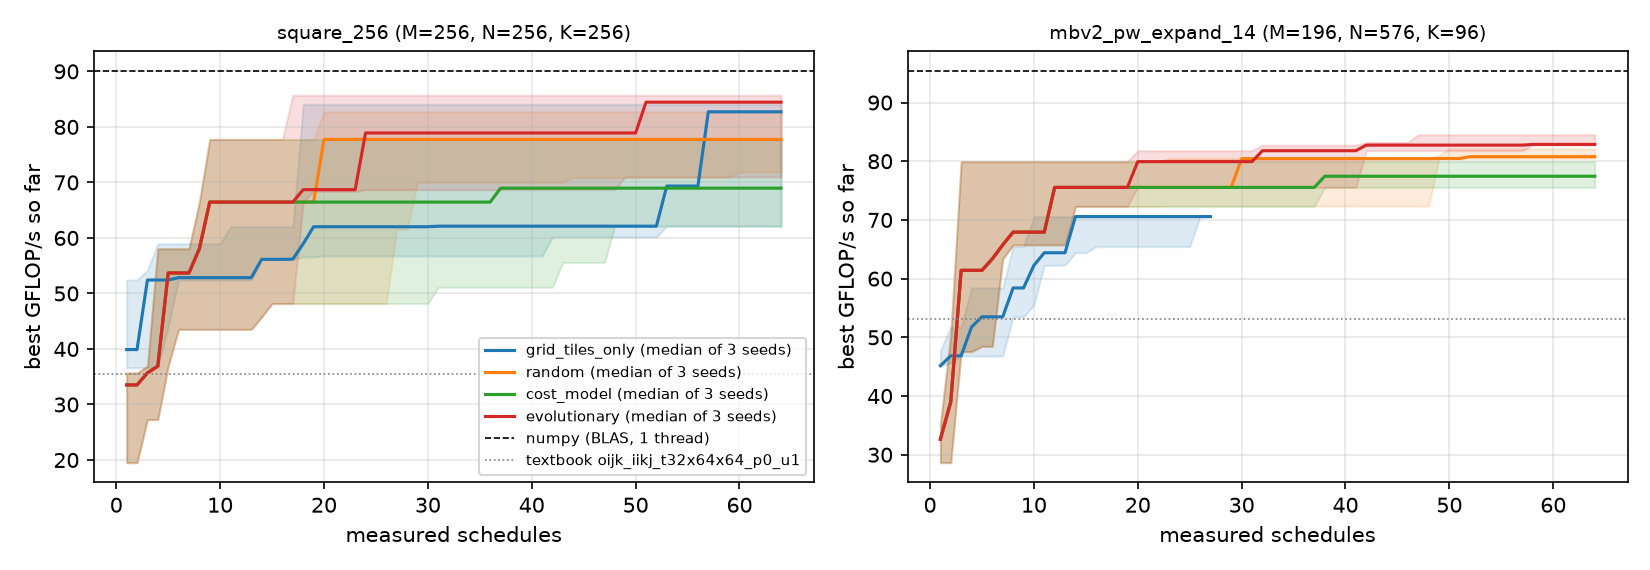
\includegraphics[width=\linewidth]{search_curves.png}
\caption{Ice Lake 上四种策略的搜索曲线。横轴是已实测的调度数，纵轴是“到目前为止最好”的 GFLOP/s；实线是 3 个种子的中位数，阴影是最小--最大。
黑色虚线是单线程 numpy，灰色点线是教科书分块。}\label{fig:curves}
\end{figure}

\Cref{fig:curves} 有四个读法。
第一，所有策略在 10 次实测以内就越过了教科书点线（35.4 / 53.1），说明教科书的默认分块离好调度很远，随便搜一下就能超过。
第二，左图（$256^3$）上进化（红）在第 24 次附近跳到约 79、第 50 次后到 84.5，最终中位数最高；grid（蓝）长期停在 62 附近，最后 10 次才跳到 82.7——它的中位数完全取决于哪个种子把好分块打乱到了前面。
第三，代价模型（绿）在两张图上都低于随机（橙）：模型引导反而让搜索停在一个平台上（\cref{sec:model}）。
第四，阴影很宽：$256^3$ 上进化的三个种子最终是 84.5、85.7、71.0，random 是 82.7、77.7、71.9；单个种子的曲线不能用来比较策略。
右图（pw\_expand\_14）的 grid 只有 27 个点，曲线在第 27 次结束；三个种子测的是同一组点、只是顺序不同，所以阴影只出现在中途，终点相同（70.6）。
三条有完整预算的曲线在 20 次之后挤在 75--83 之间。
没有任何策略达到 numpy 虚线。

\begin{table}[H]
\centering\small
\caption{各策略中位最优 GFLOP/s（括号为三个种子的最小--最大；\texttt{summary.json}）}\label{tab:main}
\setlength{\tabcolsep}{4pt}
\begin{tabular}{lrrrrrrrr}
\toprule
问题 & 空间 & 教科书 & numpy & grid & random & 代价模型 & 进化 & 全局最优 \\
\midrule
\sk{square\_256} & 30,240 & 35.4 & 90.1 & \makecell[r]{82.7\\(62.1--84.1)} & \makecell[r]{77.7\\(71.9--82.7)} & \makecell[r]{69.0\\(62.1--77.7)} & \makecell[r]{\textbf{84.5}\\(71.0--85.7)} & 85.7 \\
\addlinespace
\sk{pw\_expand\_14} & 3,888 & 53.1 & 95.4 & \makecell[r]{70.6\\(全部 27 点)} & \makecell[r]{80.8\\(80.5--82.1)} & \makecell[r]{77.4\\(75.5--79.9)} & \makecell[r]{\textbf{82.9}\\(82.7--84.5)} & 84.5 \\
\bottomrule
\end{tabular}
\end{table}

朴素 ijk 是 28.9 / 36.3 GFLOP/s，教科书分块只比它快 1.2 / 1.5 倍。进化搜索的中位最优是教科书的 $84.5/35.4=2.4$ 倍与 $82.9/53.1=1.6$ 倍，
是单线程 numpy 的 94\% 与 87\%。全局最优 85.7 / 84.5 都出自进化搜索的某个种子（\sk{ojki\_ikji\_t2x64x64\_p1\_u4} 与 \sk{ojik\_ikji\_t4x32x8\_p1\_u1}）。

\begin{table}[H]
\centering\small
\caption{达到全局最优 90\% 所需的实测次数（种子 0、1、2；— 表示 64 次内没达到）}\label{tab:trials90}
\begin{tabular}{lllll}
\toprule
问题 & grid & random & cost\_model & evolutionary \\
\midrule
\sk{square\_256} & 57、—、18 & 20、9、— & —、9、— & 24、9、— \\
\sk{pw\_expand\_14} & —、—、— & 49、30、3 & 38、—、3 & 20、42、3 \\
\bottomrule
\end{tabular}
\end{table}

\Cref{tab:trials90} 揭示了策略比较的统计困难。pw\_expand\_14 种子 2 上 random、cost\_model、evolutionary 都是 3：它们第一轮的 16 个点相同（\cref{sec:strategies}），第 3 个点就过了门槛，
所以这一个种子对比较策略没有信息。$256^3$ 种子 1 上三者都是 9，原因相同。剩下 4 个种子--问题对里，$256^3$ 种子 2 上三者都没达到；
其余 3 个中 random 两次最快（$256^3$ 种子 0 的 20、pw\_expand\_14 种子 1 的 30），进化一次最快（pw\_expand\_14 种子 0 的 20）。
按“达到 90\% 的次数”这个指标，进化并不占优；它的优势只体现在中位最优和提议质量上（\cref{tab:proposals}）。

为了估计“随机碰上一个 90\% 点有多难”，本报告用 random 策略的实测（均匀采样，无偏）另算了一个比例：$256^3$ 上 random 的 192 个不重复点里只有 2 个达到门槛（$p\approx1.0\%$），
64 次内至少命中一次的概率 $1-(1-p)^{64}\approx49\%$；pw\_expand\_14 上 190 个里有 8 个（$p\approx4.2\%$），概率约 94\%。
这与\cref{tab:trials90} 一致：$256^3$ 上 random 三个种子中有一个没命中，pw\_expand\_14 上三个都命中。

\begin{table}[H]
\centering\small
\caption{各策略提出的调度本身的质量：3 个种子全部提议的中位 GFLOP/s，以及种子 0 每轮 16 个的中位数（本报告从 \texttt{search\_history.csv} 另算）}\label{tab:proposals}
\begin{tabular}{llrl}
\toprule
问题 & 策略 & 全部提议中位 & 种子 0 的四轮中位 \\
\midrule
\multirow{4}{*}{\sk{square\_256}} & grid & 39.2 & 37.8、41.6、37.8、38.3 \\
 & random & 28.4 & 23.5、34.4、27.9、28.5 \\
 & cost\_model & 33.3 & 23.5、35.8、28.0、27.4 \\
 & evolutionary & 46.1 & 23.5、46.8、54.3、72.2 \\
\midrule
\multirow{4}{*}{\sk{pw\_expand\_14}} & grid & 46.9 & 46.5、53.1（只有 27 点） \\
 & random & 43.0 & 40.4、37.5、48.8、44.9 \\
 & cost\_model & 47.9 & 40.4、55.7、54.4、51.6 \\
 & evolutionary & 55.8 & 40.4、50.6、57.5、49.6 \\
\bottomrule
\end{tabular}
\end{table}

\Cref{tab:proposals} 换一个角度看策略：不看最好的那一个，而看它\emph{提议}的调度整体有多好。进化搜索的提议中位数最高（46.1 / 55.8），$256^3$ 种子 0 上四轮的中位数从 23.5 一路升到 72.2——
它在空间里找到了一个好调度成簇的区域，并留在那里。代价模型也把提议中位数抬高了（33.3 对 random 的 28.4），但\emph{最优值}反而更低：它改善的是平均，而不是尾部。

\begin{iqbox}{进化搜索为什么比随机好？好多少？}
好调度在空间里成簇：最内层 i 且 $t_i\le4$ 这一小块区域里集中了大部分快调度（\cref{sec:what}）。进化每次只变异一个旋钮，子代大概率留在父代所在的簇里；
$256^3$ 上进化第 2--4 轮的 144 个提议里有 91 个落在这块区域，random 只有 17 个。所以进化的提议中位数从第一轮的 23.5 升到第四轮的 72.2。
但“好多少”要谨慎：64 次预算、3 个种子下，中位最优只比 random 高 6.8 / 2.1 GFLOP/s，与单次测量噪声（$-9\%$～$+5\%$）同量级；
能区分策略的种子--问题对只有 4 个。要下更强的结论，需要更多种子，或在解析代价模型上（mlsys-infra M10，进化比随机快 1.65 倍）做无噪声对照。
\end{iqbox}

%=====================================================================
\section{结果二：什么样的调度快}\label{sec:what}

\begin{table}[H]
\centering\small
\caption{$256^3$ 上 611 个不同调度按最内层循环与 $t_i$ 分组的中位与最大 GFLOP/s（\texttt{search\_history.csv}）}\label{tab:inner}
\begin{tabular}{lrrrrrr}
\toprule
最内层 & \multicolumn{3}{c}{$t_i\le4$} & \multicolumn{3}{c}{$t_i>4$} \\
\cmidrule(lr){2-4}\cmidrule(lr){5-7}
 & 个数 & 中位 & 最大 & 个数 & 中位 & 最大 \\
\midrule
i & 137 & \textbf{52.9} & 85.7 & 65 & 10.9 & 70.0 \\
j & 154 & 39.3 & 70.0 & 131 & 38.6 & 84.1 \\
k & 78 & 21.8 & 69.5 & 46 & 11.7 & 69.0 \\
\bottomrule
\end{tabular}
\end{table}

\Cref{tab:inner} 是 E23 的直接检验。最内层 i 且 $t_i$ 小时，$t_i$ 行共享每个 B 向量，形成 $t_i\times t_j/8$ 个 ymm 累加器的寄存器块，中位数 52.9，最大 85.7；
同样最内层 i 但 $t_i$ 大时，最内层沿列访问 C（步长 $N$），无法向量化，中位数掉到 10.9——\emph{同一个循环顺序，因分块大小不同差 5 倍}。
最内层 j 是教科书写法，对 $t_i$ 不敏感（39.3 对 38.6）；它的最好点 84.1 出现在 $t_i>4$ 的 \sk{oijk\_iikj\_t16x32x8}。最内层 k 是归约维，向量化要做水平求和，两组都慢。

\begin{table}[H]
\centering\small
\caption{只看最内层 i 的调度，按 $t_i$ 细分的中位 GFLOP/s（个数）——本报告另算}\label{tab:innerti}
\begin{tabular}{lrrrrrrr}
\toprule
问题 & $t_i=1$ & 2 & 4 & 8 & 16 & 32 & 64 \\
\midrule
\sk{square\_256} & 37.2 (34) & 54.1 (59) & \textbf{63.6} (44) & 42.4 (9) & 27.2 (16) & 15.4 (18) & 7.6 (22) \\
\sk{pw\_expand\_14} & 47.3 (76) & 60.1 (63) & \textbf{63.5} (74) & -- & -- & -- & -- \\
\bottomrule
\end{tabular}
\end{table}

\Cref{tab:innerti} 把这条曲线画得更细：$t_i$ 从 1 到 4 上升（累加器从 $t_j/8$ 增到 $4t_j/8$，B 向量复用从 1 次增到 4 次），$t_i\ge8$ 后单调下降到 7.6。
峰值落在 $t_i=2$--$4$，与 E23b 的“8 到 16 个累加器”吻合：$t_j=32$ 时 $t_i=4$ 正好 16 个，$t_j=64$ 时 $t_i=2$ 正好 16 个。
pw\_expand\_14 的 $M=196$ 只允许 $t_i\in\{1,2,4\}$，正好都在好区间里，这也是它的空间虽小但分布更“好”的原因（\cref{tab:dist}）。

\begin{table}[H]
\centering\small
\caption{其余旋钮的边际效应：按取值分组的中位 GFLOP/s（个数）——本报告另算}\label{tab:knobeffect}
\begin{tabular}{lrrrr}
\toprule
问题 & 不打包 B & 打包 B & 不展开 & \texttt{unroll 4} \\
\midrule
\sk{square\_256} & 37.2 (365) & 38.9 (246) & 39.2 (381) & 33.3 (230) \\
\sk{pw\_expand\_14} & 50.3 (256) & 48.0 (234) & 52.2 (265) & 44.3 (225) \\
\bottomrule
\end{tabular}
\end{table}

打包 B 的边际效应在 $\pm2$ GFLOP/s 以内：矩阵本来就在 L2 里，B 的 tile 是否连续对 L2 → 寄存器的流量影响不大。显式 \texttt{unroll 4} 的中位数反而低 6--8 GFLOP/s：
g++ 在 \texttt{-O3} 下已经自己展开，额外的展开在最内层很短（如 $t_i=2$）时没有收益、在其他情况下增大代码。
这些是边际中位数，混杂了其他旋钮的分布（各策略采样到的子空间不同），只能说明它们不是一阶因素；最快调度里两种取值都出现过（\cref{tab:width}）。

\begin{table}[H]
\centering\small
\caption{实测调度的 GFLOP/s 分布（不同调度去重；本报告另算）}\label{tab:dist}
\begin{tabular}{lrrrrrrrr}
\toprule
问题 & 个数 & 最小 & p25 & 中位 & p75 & p90 & 最大 & $\ge$90\% 最优 \\
\midrule
\sk{square\_256} & 611 & 1.9 & 27.7 & 37.4 & 49.8 & 61.7 & 85.7 & 11（1.8\%） \\
\sk{pw\_expand\_14} & 490 & 3.7 & 36.8 & 49.0 & 62.4 & 70.2 & 84.5 & 22（4.5\%） \\
\bottomrule
\end{tabular}
\end{table}

最快与最慢差 46 / 23 倍；p90 只有最优的 72\% / 83\%。这个分布不是空间的无偏样本（进化与代价模型会集中采样好区域），所以“$\ge90\%$ 的比例”是上界；
random 的无偏估计见\cref{sec:curves}（1.0\% / 4.2\%）。

\begin{findingbox}[：瓶颈在寄存器，不在 L1]
最快的调度都是小 i 块（$t_i=2$--$4$）配 32--64 列的 j，累加器数落在 E23b 的 8--16 之间；同为最内层 i，$t_i>4$ 的中位数只有 10.9。
教科书顺序（最内层 j）只换分块也能到 84.1（\sk{t16x32x8}），默认的 $32\times64\times64$ 只有 35.4：分块大小和循环顺序一样重要。
打包 B 与显式展开都不是一阶因素。256$^3$ 的矩阵本身在 L2 里，“装进 L1”这一特征几乎不区分快慢（\cref{tab:footprint}）。
\end{findingbox}

\begin{iqbox}{分块不就是为了让数据装进 L1 吗？为什么你说 L1 不是关键？}
对这个问题不是。$256^3$ 的 A、B、C 合计 768 KiB，本来就在 1.25 MiB 的 L2 里；最快的 $t2\times64\times64$（17 KiB）和教科书的 $32\times64\times64$（32 KiB）都装得进 48 KiB 的 L1，速度却差 2.4 倍。
真正的区别在寄存器：前者 16 个 ymm 累加器、每读一个 B 向量做 2 次 FMA，循环体 32 条 FMA；后者每行 8 个累加器、每个 B 向量只用一次。
FMA 延迟 4 拍 × 2 端口要求至少 8 条独立累加链，AVX2 只有 16 个 ymm，所以好的寄存器块在 8--16 个累加器之间。
矩阵大到放不进 L2 时（例如 2048$^3$），多级缓存分块才会成为一阶因素；那时空间需要第二级 tile，本模板没有。
\end{iqbox}

%=====================================================================
\section{结果三：代价模型为什么排不准}\label{sec:model}

\begin{table}[H]
\centering\small
\caption{岭回归代价模型（\texttt{summary.json}；提议分布为本报告另算，第 2--4 轮共 144 个提议）}\label{tab:model}
\begin{tabular}{lrrrr}
\toprule
问题 & 留出 Spearman & \makecell[r]{cost\_model\\中位最优} & \makecell[r]{random\\中位最优} & \makecell[r]{提议中“最内层 j”\\的个数} \\
\midrule
\sk{square\_256} & 0.47 & 69.0 & 77.7 & 64 / 144（random 45） \\
\sk{pw\_expand\_14} & 0.53 & 77.4 & 80.8 & 58 / 144（random 45） \\
\bottomrule
\end{tabular}
\end{table}

$\rho\approx0.5$ 说明模型学到了一些东西：它把提议中位数从 random 的 28.4 / 43.0 提到 33.3 / 47.9（\cref{tab:proposals}）。但它的最优值不如 random，原因有三：

\begin{enumerate}
  \item \textbf{特征把错误的先验写死了。} 25 维里“最内层是 j”“$\log_2 t_j\times$ 最内层 j”“打包且最内层 j”三项都在编码教科书的“j 最内层可向量化”。
  模型于是偏向最内层 j：$256^3$ 上第 2--4 轮 144 个提议里 64 个最内层是 j，random 只有 45 个；而最快的调度最内层是 i（\cref{tab:inner}）。
  \item \textbf{线性模型表达不了关键交互。} “最内层 i 好”只在 $t_i\le4$ 时成立，$t_i>4$ 时最内层 i 是最差的一组（10.9）。这是一个符号随 $t_i$ 翻转的交互，
  一个线性模型只能给“最内层 i”一个平均系数，而这个平均值被 $t_i>4$ 的 65 个慢点拉低。
  \item \textbf{数据太少。} 64 次预算下第一轮只有 16 个随机点训练模型，第二轮 32 个；25 维特征加截距，前两轮几乎是在用噪声拟合。
\end{enumerate}

\emph{整体}秩相关与\emph{头部}精度也不是一回事。$\rho$ 主要由占多数的中间点决定：只要能把 2 GFLOP/s 和 50 GFLOP/s 分开，$\rho$ 就不会低；
而搜索需要的是在 1\%--4\% 的头部里分出谁更好，那里点之间只差几个 GFLOP/s，模型误差和测量噪声都比这大。
mlsys-infra 的 Triton matmul 上实验室代价模型的 $\rho$ 为 0.65 / 0.36 / 0.10，同一量级。

\begin{iqbox}{AutoTVM 有代价模型，为什么最后还要在设备上实测？}
代价模型只是筛子，不是裁判。这里的岭回归留出 $\rho$ 只有 0.47 / 0.53，在 64 次预算下中位最优甚至不如随机；即使模型更好（XGBoost、MLP），它也只负责从几千个候选里挑出值得测的十几个。
最终选择必须实测，而实测本身有 5\% 级噪声，所以还要复测（\cref{sec:noise}）。
改进方向是让特征表达真正的瓶颈：加“$t_i\le4$ 且最内层 i”“累加器数 $t_i t_j/8$”这类交互特征，或换树模型自动发现交互；
Ansor 的做法是从生成的低层程序里抽特征（每个 buffer access 的步长、复用距离），而不是从高层旋钮抽。
\end{iqbox}

%=====================================================================
\section{结果四：噪声与赢家诅咒}\label{sec:noise}

\begin{table}[H]
\centering\small
\caption{前 8 名复测（256 位列；\texttt{vector\_width.csv}）}\label{tab:remeasure}
\begin{tabular}{lrrrr}
\toprule
问题 & 搜索时前 8 平均 & 复测平均 & 单个调度复测相对搜索 & 第一名 搜索 → 复测 \\
\midrule
\sk{square\_256} & 83.3 & 80.5 & $-8.9\%$～$+4.6\%$ & 85.7 → 80.1 \\
\sk{pw\_expand\_14} & 82.4 & 77.8 & $-8.7\%$～$-0.2\%$ & 84.5 → 79.8 \\
\bottomrule
\end{tabular}
\end{table}

复测平均低 3.3\% / 5.6\%，单个调度在 $-9\%$～$+5\%$ 之间变化。8 个点里 $256^3$ 有 5 个、pw\_expand\_14 有全部 8 个变低：
这是赢家诅咒的典型形态——被选进前 8 的点，往往是那次测量恰好偏高的点。搜索里的第一名 85.7 复测是 80.1，降了 6.5\%；
复测里最快的反而是搜索中排第 3 的 \sk{oijk\_ijki\_t4x256x8\_p1\_u4}（87.5）。pw\_expand\_14 上复测第一名 \sk{ojik\_ikji\_t4x32x16\_p1\_u4}（80.7）在搜索中排第 8。

前 8 名的搜索值本身只相差 8\%（78.9--85.7），比单次噪声的范围还小，\emph{名次没有意义}。上一次完整运行（同一代码、同一机器）pw\_expand\_14 的 27 点 grid 最优是 77.5，这次 70.6，也是这个量级（笔记 M06）。
所以\cref{sec:curves}里策略之间的几个 GFLOP/s 差距，在这个噪声水平和 3 个种子下并不显著。

\begin{findingbox}[：报告最优值之前必须复测]
从几百个带噪声的测量里挑最大值，最大值本身就偏高：前 8 名复测平均低 3\%--6\%，第一名低 6.5\%。比较策略要用多个种子的中位数和“达到 90\% 的次数”，
报告最优调度要换一个二进制复测；前几名之间的名次差小于噪声时，应当把它们视为并列，按其他标准（代码大小、编译时间、对形状的鲁棒性）选。
\end{findingbox}

\begin{iqbox}{你的搜索报告最优 85.7 GFLOP/s，这个数能写进论文吗？}
不能直接写。它是 600 多个带噪声测量的最大值，复测只有 80.1。应当报告复测值，并说明复测协议（重新编译、单独运行、重复次数、取中位数）。
更稳健的做法是对前 $k$ 名各做多次独立复测，用复测均值重新排序；TVM 的 tuning log 里每条记录也保存多次运行的结果。
另外要声明测量环境：这里是虚拟机，频率与邻居负载不受控，噪声比裸机大；本实验只并行编译、严格顺序运行，就是为了不让测量互相抢 L2/L3 和功耗预算。
\end{iqbox}

%=====================================================================
\section{结果五：256 位与 512 位向量}\label{sec:width}

\begin{table}[H]
\centering\small
\caption{Ice Lake 前 8 名用两种向量宽度编译（GFLOP/s；\texttt{vector\_width.csv}）}\label{tab:width}
\begin{tabular}{llrrr}
\toprule
问题 & 调度 & 256 位 & 512 位 & 512 / 256 \\
\midrule
\multirow{8}{*}{\sk{square\_256}}
 & \sk{ojki\_ikji\_t2x64x64\_p1\_u4} & 80.1 & 55.7 & 0.70 \\
 & \sk{okij\_ikji\_t2x64x32\_p1\_u1} & 77.5 & 55.3 & 0.71 \\
 & \sk{oijk\_ijki\_t4x256x8\_p1\_u4} & 87.5 & 82.9 & 0.95 \\
 & \sk{oijk\_iikj\_t16x32x8\_p0\_u1} & 77.8 & \textbf{81.1} & 1.04 \\
 & \sk{ojki\_ikji\_t2x64x32\_p1\_u1} & 78.1 & 53.0 & 0.68 \\
 & \sk{oijk\_iikj\_t64x32x8\_p0\_u1} & 83.5 & 69.7 & 0.84 \\
 & \sk{oikj\_ijki\_t4x64x8\_p1\_u4} & 85.8 & 76.3 & 0.89 \\
 & \sk{oikj\_ijki\_t4x64x8\_p0\_u1} & 74.2 & 69.2 & 0.93 \\
\midrule
\multirow{8}{*}{\sk{pw\_expand\_14}}
 & \sk{ojik\_ikji\_t4x32x8\_p1\_u1} & 79.8 & 56.2 & 0.70 \\
 & \sk{oikj\_ijik\_t4x16x8\_p0\_u1} & 80.6 & 63.6 & 0.79 \\
 & \sk{ojki\_ikij\_t1x32x8\_p0\_u1} & 78.2 & 74.8 & 0.96 \\
 & \sk{ojki\_ikji\_t2x64x32\_p1\_u4} & 77.1 & 54.3 & 0.70 \\
 & \sk{oikj\_ijki\_t4x32x8\_p1\_u4} & 75.3 & \textbf{82.4} & 1.09 \\
 & \sk{ojki\_iikj\_t1x32x8\_p0\_u1} & 77.0 & \textbf{77.2} & 1.00 \\
 & \sk{okji\_ikji\_t2x64x16\_p1\_u1} & 73.9 & 54.4 & 0.74 \\
 & \sk{ojik\_ikji\_t4x32x16\_p1\_u4} & 80.7 & 57.3 & 0.71 \\
\bottomrule
\end{tabular}
\end{table}

\begin{table}[H]
\centering\small
\caption{向量宽度汇总}\label{tab:widthsum}
\begin{tabular}{lrrrr}
\toprule
问题 & 256 位中位 & 512 位中位 & 512 位更快 & 512/256 比值中位 \\
\midrule
\sk{square\_256} & 79.1 & 69.5 & 1 / 8 & 0.86 \\
\sk{pw\_expand\_14} & 77.7 & 60.5 & 2 / 8 & 0.76 \\
\bottomrule
\end{tabular}
\end{table}

16 个候选里 13 个用 512 位更慢，中位数低 12\% / 22\%。损失最大的一组很有规律：内层顺序为 kji（key 里的 \sk{\_ikji\_}，ii 最内、jj 在其上）的 7 个调度，
比值全部在 0.68--0.74，也就是 256 位下最典型的“$t_i$ 行 × 若干 ymm”寄存器块结构；其余 9 个调度的比值在 0.79--1.09，损失小得多，3 个反而变快。
\sk{ojki\_ikji\_t2x64x64\_p1\_u4} 用 512 位编译后循环体从 32 条 ymm FMA 变成 16 条 zmm FMA，指令数减半，GFLOP/s 却从 80.1 掉到 55.7。

频率只解释一部分：2.42 / 2.8 GHz 最多 14\%，而这一组掉了约 30\%。一个可能的原因是寄存器块形状改变：$t_j=64$ 用 zmm 时只有 4 个向量宽，$2\times4=8$ 个累加器，
落到 E23b 的下限，FMA 流水刚好喂满、没有余量；但这只是推测，虚拟机里没有性能计数器，其余约 20\% 没有定位。

\begin{iqbox}{为什么 GCC 在 AVX-512 机器上默认不用 512 位向量？}
两个原因。第一，AVX-512 重负载会降频：这台 Ice Lake 上 zmm 峰值对应 2.42 GHz，而 256 位代码能跑到更高频率（系统报告最高 2.8 GHz），降频还会拖慢同核上的标量代码；
第二，很多自动向量化的循环用不满 512 位（短循环、余数处理、gather/scatter），宽度翻倍只换来更大的尾部开销。实测这台机器上 13/16 个候选用 512 位变慢。
但这个默认值不是普适真理：同一批搜索在 Sapphire Rapids 上 16/16 都是 512 位更快（\cref{sec:xeon}）。所以向量宽度本身应当是一个按目标机器搜索的旋钮，
就像 TVM 对每个 target 单独保存调优日志。
\end{iqbox}

%=====================================================================
\section{结果六：Xeon 8470Q 复现——最优点换了位置}\label{sec:xeon}

\begin{figure}[H]
\centering
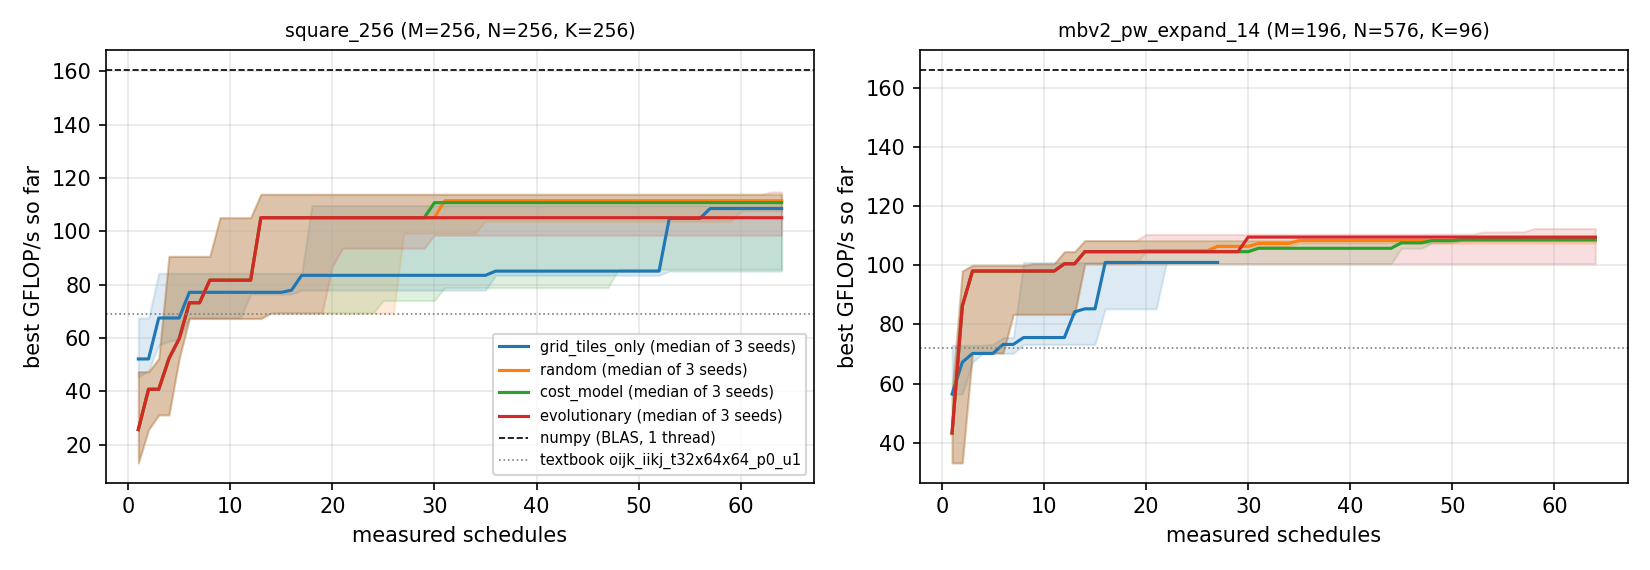
\includegraphics[width=\linewidth]{xeon8470q/search_curves.png}
\caption{Xeon 8470Q 上重跑全部四种搜索 × 3 个种子的搜索曲线（图例同\cref{fig:curves}）。黑色虚线是单线程 numpy（约 161 / 166 GFLOP/s），所有策略都离它很远。}\label{fig:xeon}
\end{figure}

\Cref{fig:xeon} 与\cref{fig:curves} 的形状不同。第一，纵轴整体上移：教科书点线在 69 / 72 附近，搜索曲线在 105--115 收敛；numpy 虚线升到 160 以上，与搜索的差距从 Ice Lake 的约 6\% 拉大到约 30\%。
第二，曲线收敛得更快、更紧：$256^3$ 上进化在第 13 次附近就到约 105，random 与 cost\_model 在第 30 次附近到约 110，pw\_expand\_14 上三条曲线在第 3 次就跳到约 97，之后在 100--110 之间几乎重合。
这与无偏估计一致：Xeon 上 random 的提议里达到 90\% 门槛的比例是 4.7\% / 6.3\%，比 Ice Lake 的 1.0\% / 4.2\% 高，好调度更“多”，搜索更容易。
第三，grid（蓝）依然最差，并且在 $256^3$ 上同样要到第 50 次之后才跳上去。

\begin{table}[H]
\centering\small
\caption{本地 Ice Lake 与服务器 Xeon 8470Q（\texttt{summary.json} 与 \texttt{xeon8470q/summary.json}）}\label{tab:xeon}
\setlength{\tabcolsep}{3.5pt}
\begin{tabular}{lrrrrrr}
\toprule
问题 & \makecell[r]{最优\\本地 → 服务器} & \makecell[r]{numpy 1 线程\\本地 → 服务器} & \makecell[r]{random 到 90\%\\（种子 0）} & \makecell[r]{代价模型\\Spearman} & \makecell[r]{前 8 名\\256 位最优} & \makecell[r]{前 8 名\\512 位最优} \\
\midrule
\sk{square\_256} & 85.7 → 114.7 & 90.1 → 160.6 & 20 → 13 & 0.47 → 0.54 & 115.1 & \textbf{173.1} \\
\sk{pw\_expand\_14} & 84.5 → 112.4 & 95.4 → 166.1 & 49 → 14 & 0.53 → 0.56 & 111.1 & \textbf{156.5} \\
\bottomrule
\end{tabular}
\end{table}

\begin{table}[H]
\centering\small
\caption{Xeon 8470Q 上各策略中位最优 GFLOP/s（括号为三个种子范围）}\label{tab:xeonmain}
\begin{tabular}{lrrrrrr}
\toprule
问题 & 教科书 & grid & random & 代价模型 & 进化 & 全局最优 \\
\midrule
\sk{square\_256} & 69.1 & \makecell[r]{108.5\\(85.1--109.7)} & \makecell[r]{\textbf{111.5}\\(107.6--113.9)} & \makecell[r]{110.7\\(85.7--113.9)} & \makecell[r]{105.1\\(98.5--114.7)} & 114.7 \\
\addlinespace
\sk{pw\_expand\_14} & 72.2 & \makecell[r]{101.0\\(全部 27 点)} & \makecell[r]{108.3\\(107.4--109.0)} & \makecell[r]{108.7\\(108.3--109.7)} & \makecell[r]{\textbf{109.5}\\(100.5--112.4)} & 112.4 \\
\bottomrule
\end{tabular}
\end{table}

在 Xeon 上，策略之间的排名变了：$256^3$ 上 random（111.5）中位最高，进化（105.1）反而最低；pw\_expand\_14 上进化以 109.5 略高。
三个有完整预算的策略中位数相差不到 7\%，与 Ice Lake 上复测噪声的范围相当——换一台机器“哪个策略最好”就不同，这本身说明 3 个种子下的策略差距不显著。

\subsection{向量宽度的结论翻转}

\begin{table}[H]
\centering\small
\caption{Xeon 8470Q 前 8 名用两种向量宽度编译（\texttt{xeon8470q/vector\_width.csv}；比值为本报告另算）}\label{tab:xeonwidth}
\begin{tabular}{lrrrr}
\toprule
问题 & 256 位中位 & 512 位中位 & 512 位更快 & 512/256 比值（最小--最大） \\
\midrule
\sk{square\_256} & 112.4 & 166.8 & 8 / 8 & 1.47（1.38--1.58） \\
\sk{pw\_expand\_14} & 108.6 & 147.5 & 8 / 8 & 1.37（1.33--1.56） \\
\bottomrule
\end{tabular}
\end{table}

本地 Ice Lake 上 512 位只有 3/16 更快、中位数慢 12\%--22\%；Sapphire Rapids 上 16/16 更快，最优 173.1 对 115.1、156.5 对 111.1。
SPR 的 AVX-512 降频档位比 Ice Lake 温和得多，且有两个完整的 512 位 FMA 端口。值得注意的是，512 位复测的 173.1 已经超过 numpy 单线程的 160.6——
但这是两种编译参数、两次独立测量的比较，而且搜索本身是在 256 位下做的；如果在 512 位下重新搜索，最优调度可能又不同。

\subsection{最优调度可不可以迁移}

\begin{table}[H]
\centering\small
\caption{两台机器都测过的调度上的交叉比较（本报告从两份 \texttt{search\_history.csv} 另算）}\label{tab:cross}
\setlength{\tabcolsep}{4pt}
\begin{tabular}{lrrrrr}
\toprule
问题 & \makecell[r]{共同\\调度} & \makecell[r]{排序\\Spearman} & \makecell[r]{服务器 / 本地\\加速比中位（范围）} & \makecell[r]{本地最快者\\在服务器的名次} & \makecell[r]{服务器最快者\\在本地的名次} \\
\midrule
\sk{square\_256} & 372 & 0.86 & \makecell[r]{1.40\\(0.30--5.44)} & \makecell[r]{3\\(服务器最优的 96\%)} & \makecell[r]{232\\(本地最优的 39\%)} \\
\addlinespace
\sk{pw\_expand\_14} & 319 & 0.89 & \makecell[r]{1.39\\(0.49--2.45)} & \makecell[r]{16\\(95\%)} & \makecell[r]{165\\(54\%)} \\
\bottomrule
\end{tabular}
\end{table}

共同调度来自两台机器上相同的随机采样（random 与各策略第一轮在同一种子下完全相同），以及搜索碰巧都访问过的点。\Cref{tab:cross} 给出一个比 README 更细的图景：

\begin{itemize}
  \item \textbf{整体排序高度可迁移。} 两台机器上的秩相关 0.86 / 0.89，远高于代价模型的 0.47 / 0.53。“另一台机器上的实测”是比手写特征好得多的代价模型——这正是 TVM 的迁移学习（用别的设备的 tuning log 预训练代价模型）的依据。
  \item \textbf{最优点不可迁移。} 两台机器各自的前 8 名只重合 3 / 1 个；共同调度里服务器最快的 \sk{oikj\_iikj\_t64x32x8\_p0\_u4}（113.9）在本地只排第 232、33.0 GFLOP/s，是本地最优的 39\%。
  本地前 8 名多是 \sk{ikji} / \sk{ijki} 内层顺序、64 宽的 tile（如 \sk{ojki\_ikji\_t2x64x64}），服务器前 8 名有 7 个是 \sk{iikj} 内层、32$\times$8 tile。
  \item \textbf{反方向迁移要好得多。} 共同调度里本地最快的那个，在服务器上（共同调度中）仍排第 3 / 第 16，达到服务器全局最优的 95\% 以上；反过来却只有 39\% / 54\%。不对称性来自加速比的范围：同一调度换机器，快 5.4 倍到慢 3.3 倍都有。
\end{itemize}

\begin{iqbox}{在一台机器上调好的调度，部署到另一台同为 x86 AVX-512 的机器上能直接用吗？}
不能直接用，但也不用从零开始。这里两台机器（Ice Lake 与 Sapphire Rapids）在 300 多个共同调度上的排序 Spearman 有 0.86--0.89，所以别的机器的调优日志是很好的先验：
用它预训练代价模型或作为进化搜索的初始种群，能大幅减少实测次数。但最优点换了位置：服务器最优在本地只有本地最优的 39\%，前 8 名几乎不重合；
连“要不要开 512 位向量”这种二元选择都会翻转。所以 AutoTVM / Ansor 要在目标设备上测量，并为每种硬件单独保存调优日志；
端侧部署时离线在同型号设备上搜索，把（形状，最优调度）存进调度库，设备上只查表。
\end{iqbox}

\begin{findingbox}[：模板的天花板]
两台机器上搜索器的最优都低于 numpy：Ice Lake 上差 6\% / 13\%，Xeon 上差约 30\%（114.7 对 160.6）。模板没有打包 B 到寄存器块形状、没有 K 方向的寄存器分块、没有显式微内核；
g++ 自动向量化出来的内核在频率更高、端口更多的 SPR 上暴露出更大的差距。搜索只能在空间内部找最优，空间的天花板由模板决定——这是 Ansor 用 sketch 生成更丰富结构的动机。
\end{findingbox}

%=====================================================================
\section{结论}

\begin{findingbox}[：五条主要结论]
\begin{enumerate}[label=(\alph*)]
  \item 搜索有效：64 次实测、3 个种子，进化搜索的中位最优是教科书分块的 2.4 / 1.6 倍，达到单线程 numpy 的 94\% / 87\%。
  \item 好调度由最内层的硬件资源决定：16 个 ymm 寄存器、4 拍 × 2 端口的 FMA 流水；最内层 i 且 $t_i=2$--$4$ 的寄存器块最快，L1 足迹不是区分变量。
  \item 手写特征的代价模型受限于特征：把“j 最内层”的先验写进特征，模型就学不到反例；留出 $\rho$ 0.47 / 0.53，中位最优不如随机。
  \item 噪声与策略差距同量级：复测 $-9\%$～$+5\%$，前 8 名平均低 3\%--6\%；策略比较只能看多种子中位数与达到 90\% 的次数，而且在 3 个种子下并不显著。
  \item 调优结果绑定硬件：向量宽度的最优选择在 Ice Lake 与 Sapphire Rapids 上相反；两台机器整体排序相关 0.86 / 0.89，但前 8 名几乎不重合。
\end{enumerate}
\end{findingbox}

\section{20 秒讲法}

我在 4 核 CPU 上自己做了一遍 AutoTVM：把 GEMM 的循环顺序、分块、布局、展开做成 3 万个点的空间，生成 C++ 实测，比较四种搜索策略。
进化搜索 64 次实测就把教科书分块提速 2.4 倍，接近 numpy；最快的调度是 2--4 行 × 64 列的寄存器块，不是 L1 分块。
但有三个反直觉的结果：岭回归代价模型排序相关只有 0.5、还不如随机；搜索报告的最优值复测低 6.5\%，前几名的名次没有意义；
强制 512 位向量在 Ice Lake 上让 13/16 个调度变慢，在 Sapphire Rapids 上却全部快 1.3--1.6 倍——调度必须在目标机器上测。

\begin{caveatbox}
\begin{itemize}
  \item 单次实测有 $-9\%$～$+5\%$ 的波动，前几名之间的名次没有意义；策略之间几个百分点的差距在 3 个种子、64 次预算下也不显著（Xeon 上策略排名就与 Ice Lake 不同）。
  \item “512 位更慢”只对这些 g++ 自动向量化出来的内核、只在这台 Ice Lake 虚拟机上成立；手写的 AVX-512 微内核（例如 OpenBLAS / oneDNN）可以用满 zmm，Sapphire Rapids 上结论相反。
  \item numpy 的 90 / 161 GFLOP/s 是它自带的 BLAS，本仓库没有核对它用的指令集；“搜索器接近 / 超过 numpy”只是同机同尺寸的参照，不是内核层面的对比。
  \item 512 位比 256 位多出的约 20\% 损失没有定位：虚拟机里没有性能计数器；“寄存器块形状变化”只是推测。
  \item 空间是一个固定模板（AutoTVM 风格），只搜单线程，没有多线程并行、多级缓存分块和 Ansor 的 sketch 生成；结论不推广到放不进 L2 的大矩阵。
  \item 分组中位数（\cref{tab:inner,tab:innerti,tab:knobeffect,tab:dist}）来自搜索访问过的调度，不是空间的无偏样本；旋钮的边际效应混杂了其他旋钮的分布。
  \item 跨机器的交叉比较（\cref{tab:cross}）只在两台机器都碰巧测过的 372 / 319 个调度上，且两台机器的编译器版本与操作系统不同，不能把差异全部归因于微架构。
\end{itemize}
\end{caveatbox}

%=====================================================================
\section{复现}

\begin{lstlisting}[language=bash,numbers=none]
cd solutions/mlc/tensor-program-tuning
python -m pytest -q tests
python scripts/run_experiments.py               # 2 problems x 4 strategies x 3 seeds + re-measurement; idle machine,
                                                # about 3 minutes when the compile cache in cpp/bin/ hits
python scripts/run_experiments.py --seeds 1     # quick version
python scripts/run_experiments.py --budget 32   # smaller budget per strategy and seed
\end{lstlisting}

需要 g++（MinGW 或 Linux 均可）。编译 4 路并行，运行严格顺序；二进制按“源码 + 编译参数”的哈希缓存在 \texttt{cpp/bin/}（不入库）。
输出写到 \nolinkurl{artifacts/raw/}（\texttt{summary.json}、\texttt{search\_history.csv}、\texttt{vector\_width.csv}）与 \nolinkurl{artifacts/figures/search_curves.png}；
Xeon 8470Q 的结果在 \nolinkurl{artifacts/raw/xeon8470q/} 与 \nolinkurl{artifacts/figures/xeon8470q/}。
本报告中标注“另算”的表格由这三份原始文件直接分组统计得到，没有新的测量。


\begin{thebibliography}{99}
\bibitem{halide} J.~Ragan-Kelley, C.~Barnes, A.~Adams, et al. Halide: A Language and Compiler for Optimizing Parallelism, Locality, and Recomputation in Image Processing Pipelines. \emph{PLDI}, 2013.
\bibitem{autotvm} T.~Chen, L.~Zheng, E.~Yan, et al. Learning to Optimize Tensor Programs. \emph{NeurIPS}, 2018.
\bibitem{ansor} L.~Zheng, C.~Jia, M.~Sun, et al. Ansor: Generating High-Performance Tensor Programs for Deep Learning. \emph{OSDI}, 2020.
\bibitem{xgboost} T.~Chen, C.~Guestrin. XGBoost: A Scalable Tree Boosting System. \emph{KDD}, 2016.
\bibitem{tvm} T.~Chen, T.~Moreau, Z.~Jiang, et al. TVM: An Automated End-to-End Optimizing Compiler for Deep Learning. \emph{OSDI}, 2018.
\bibitem{mobilenetv2} M.~Sandler, A.~Howard, M.~Zhu, A.~Zhmoginov, L.-C.~Chen. MobileNetV2: Inverted Residuals and Linear Bottlenecks. \emph{CVPR}, 2018.
\end{thebibliography}

\end{document}
